Når vi spesifiserer egenskapene til en sensor skiller vi mellom presisjon
og nøyaktighet.

Presisjon sier hvor stor spredning det er.
Høy presisjon betyr liten spredning.

Nøyaktighet sier hvor nærme målet man er.
Stor nøyaktighet kan ha mye variasjon, men variasjonene er sentrert rundt
det riktige området.

\begin{figure}[H]
  \centering
  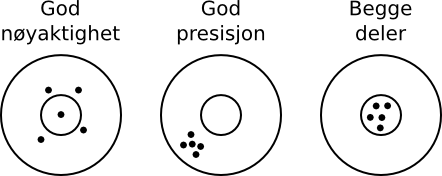
\includegraphics[width=0.67\textwidth]{./img/presisjon}
  \caption{Presisjon vs Nøyaktighet}
\end{figure}

Nøyaktighet kan sies å representere systemavvik og
presisjon tilfeldighet.

\begin{figure}[H]
  \centering
  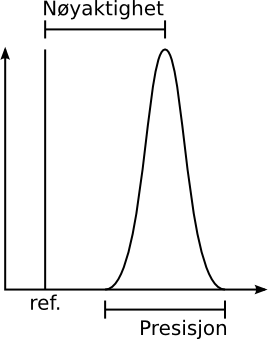
\includegraphics[width=0.33\textwidth]{./img/avvik}
  \caption{Presisjon/nøyaktighet grafert}
\end{figure}
